\documentclass[tikz]{standalone}
\usepackage{amsmath}
\usetikzlibrary{arrows, automata, positioning, calc}
\begin{document}

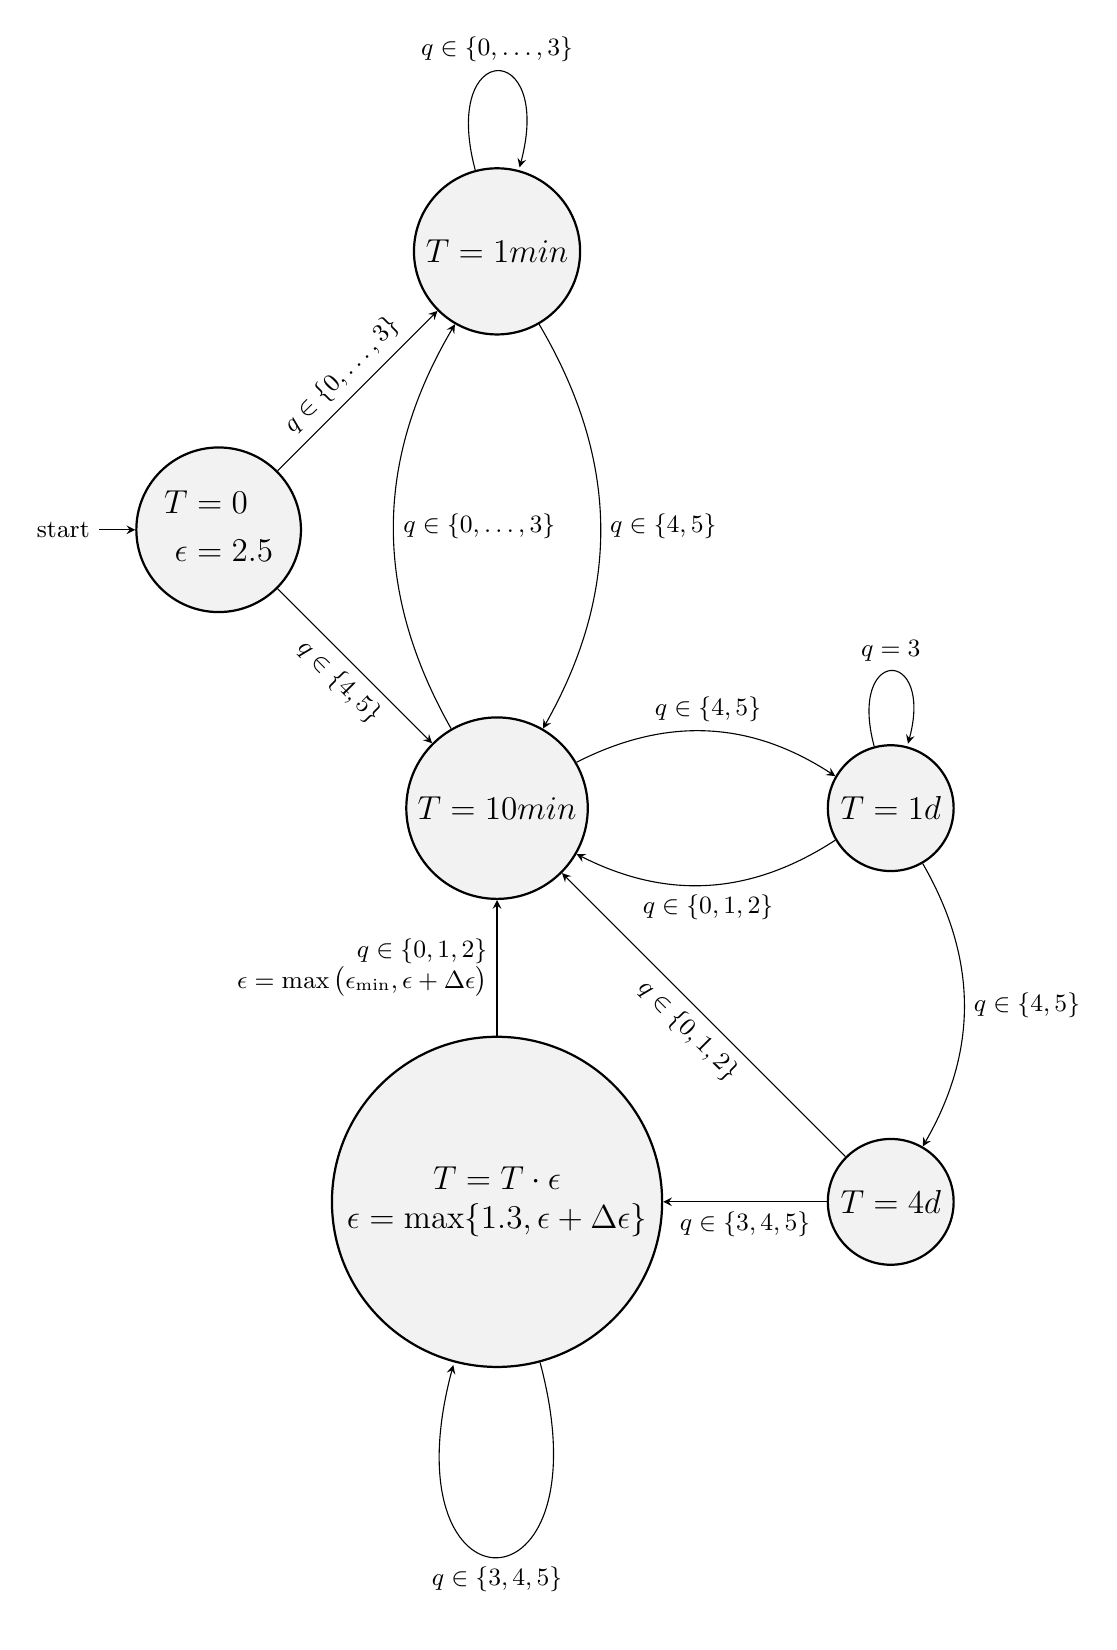
\begin{tikzpicture}[
    ->,  % makes the edges directed
    >=stealth,
    node distance=5cm, % specifies the minimum distance between two nodes. Change if necessary.
    every node/.style={font={\small}}, % sets the properties for each ’state’ node
    every state/.style={thick, fill=gray!10, font={\large}}, % sets the properties for each ’state’ node
  ]

  \node[state, initial] (q1) {
    $\begin{aligned}
      T &= 0\\
      \epsilon &= 2.5
    \end{aligned}$
  };
  \node[state, above right of=q1] (q2) {$T = 1min$};
  \node[state, below right of=q1] (q3) {$T = 10min$};
  \node[state, right of=q3] (q4) {$T = 1d$};
  \node[state, below of=q4] (q5) {$T = 4d$};
  \node[state, left of=q5, align=center] (q6) {%
    $T = T \cdot \epsilon$ \\
    $\epsilon = \max\{1.3, \epsilon + \Delta \epsilon \}$
  };

  \draw (q1) edge[sloped, anchor=center, above] node{$q \in \{0, \ldots, 3\}$} (q2);
  \draw (q1) edge[sloped, anchor=center, below] node{$q \in \{4, 5\}$} (q3);
  \draw (q2) edge[bend left, right] node{$q \in \{4, 5 \}$} (q3);
  \draw (q2) edge[loop above] node{$q \in \{0, \ldots, 3 \}$} (q2);
  \draw (q3) edge[bend left, right] node{$q \in \{0, \ldots, 3 \}$} (q2);
  \draw (q3) edge[bend left, above] node{$q \in \{4, 5\} $} (q4);
  \draw (q4) edge[bend left, below] node{$q \in \{0, 1, 2\} $} (q3);
  \draw (q4) edge[loop above] node{$q = 3$} (q4);
  \draw (q4) edge[bend left, right] node{$q \in \{4, 5 \}$} (q5);
  \draw (q5) edge[below] node{$q \in \{3, 4, 5\}$} (q6);
  \draw (q5) edge[sloped, anchor=center, below] node{$q \in \{0, 1, 2\}$} (q3);
  \draw (q6) edge[loop below] node{$q \in \{3, 4, 5\}$} (q6);
  \draw (q6) edge[left, align=right] node{
    $q \in \{0, 1, 2\}$ \\
    $\epsilon = \max\big(\epsilon_\text{min}, \epsilon+\Delta \epsilon \big)$} (q3);

\end{tikzpicture}

\end{document}
